
%!TeX program = XeLaTeX
\documentclass[12pt, a4paper, twocolumn]{article} 
%\usepackage[no-math]{xeCJK} %For Traditional Chinese in XeLaTeX
%\setCJKmainfont{MingLiU} %For Traditional Chinese in XeLaTeX
%\setCJKsansfont{Microsoft JhengHei} %For Traditional Chinese in XeLaTeX

% *** MISC UTILITY PACKAGES ***
%
\usepackage{listings}
\usepackage[english]{babel}
\usepackage{placeins}
%\usepackage{ifpdf}
% Heiko Oberdiek's ifpdf.sty is very useful if you need conditional
% compilation based on whether the output is pdf or dvi.
% usage:
% \ifpdf
%   % pdf code
% \else
%   % dvi code
% \fi

% *** GRAPHICS RELATED PACKAGES ***
%
%\usepackage[pdftex]{graphicx}
\usepackage{graphicx}
% declare the path(s) where your graphic files are
\graphicspath{{./Figures/}{../Figures/}{../}{../../}} 
% and their extensions so you won't have to specify these with
% every instance of \includegraphics
\DeclareGraphicsExtensions{.pdf,.jpeg,.png}

% *** MATH PACKAGES ***
%
\usepackage[cmex10]{amsmath}

%\interdisplaylinepenalty=2500
% after loading amsmath to restore such page breaks as IEEEtran.cls normally
% does. amsmath.sty is already installed on most LaTeX systems. The latest
% version and documentation can be obtained at:
% http://www.ctan.org/tex-archive/macros/latex/required/amslatex/math/
\usepackage{amssymb,amsfonts} %Added to get math
\usepackage{amsthm} % Added to get theorems
\usepackage{mathtools} % Added to get \mathclap working
%\usepackage{bbold} % Defines \mathbb{} for numbers but also changes to a sans serif font for captial letters
%\usepackage{doublestroke} % Defines \mathds{} which I use to get symbol for vector with ones (Too complicated installation so skip)
\usepackage{bbm} % Defines \mathbbm{} which I use to get symbol for vector with ones


% *** FLOAT PACKAGES ***
%
\usepackage{paralist} % Inline list used in box
\usepackage{lipsum,framed} % Needed to create box and my comments
\usepackage{color} %Needed for color, the option usenames,dvipsnames will define a set of basic colors.
\usepackage[table]{xcolor} %Needed to color rows in table
%\usepackage[config, font={small}, labelfont={bf}, margin={3mm}]{caption, subfig} %Modifies the look of the captions of floats (may cause conflict with memoir class)
%\usepackage[config, margin={3mm}, font={small}, labelfont={bf}]{caption}%Modifies the look of the captions of floats (may cause conflict with memoir class)
\usepackage{subcaption}
%\usepackage{rotating} %Add to rotate figures and tables in PDF file
%\usepackage{filecontents} %Adds ability to compile separate files from within tex code, used for Practical_collinearity_for_column_uncertainty_proof_illustration_All.pdf generation

% Tabular packages
%\usepackage{longtable}
%\usepackage{multirow} % Add to get multirow working in tabular
%\usepackage{arydshln} %Add to get dashed lines working in tabular
%\usepackage{booktabs} %Commands for enhancing quality of tables
%\usepackage{adjustbox} %Handy for resizing tables
\usepackage{diagbox} % split cell daigonally
\usepackage[para,online,flushleft]{threeparttable}

\usepackage{ifdraft} %Enables \ifdraft{draft case}{final case} where things automatically are turned on and off depending on draft status.
\usepackage{comment} %Used to get comments turned on or off.
\usepackage{xspace} %Added to get automatic spacing after e.g., etc.
\usepackage{setspace} % Added to get todo boxes working (needed for \singlespacing) N
%\usepackage{makeidx} %Used to generate index
%\makeindex %Needed to tell Latex to make the index
%% Need to run command makeindex %.idx 
%\usepackage[intoc]{nomencl} %Can be used to generate abbreviations list but produces multiple entries if defined more than once, so glossaries is recomended.
%\renewcommand{\nomname}{Abbreviations}
%\makenomenclature %Needed to tell Latex to make the abbreviations list
%% Need to run command makeindex %.nlo -s nomencl.ist -o %.nls
%makeindex Nordling_PhD_thesis_main.nlo -s nomencl.ist -o Nordling_PhD_thesis_main.nls
\usepackage{etex} % Added to be able to use tikz
\usepackage{tikz} % Added to get todo boxes (must be after graphicx and color)
%\usepackage[final]{microtype} %Function unknown added by Per Sahlholm
%\usepackage{marvosym} %Function unknown added by Per Sahlholm
%\usepackage[table]{xcolor} %Function unknown added by Per Sahlholm causes option clash.
\usepackage[final]{pdfpages} %Package for inserting PDF documents in generated document.
\usepackage{enumitem} %Change numbering in lists

% *** PDF, URL AND HYPERLINK PACKAGES ***
%
\usepackage{url}
% url.sty was written by Donald Arseneau. It provides better support for
% handling and breaking URLs. url.sty is already installed on most LaTeX
% systems. The latest version and documentation can be obtained at:
% http://www.ctan.org/tex-archive/macros/latex/contrib/url/
% Basically, \url{my_url_here}.
% Special hack below to break the damn URL!
\def\UrlBreaks{\do\.\do\@\do\\\do\/\do\!\do\_\do\|\do\;\do\>\do\]%
	\do\)\do\,\do\?\do\'\do+\do\=\do\#\do\i\do\m\do\t\do\a\do\x}%
\urlstyle{rm} %
\usepackage[bookmarks=true,bookmarksnumbered=true,hypertexnames=true,breaklinks=true,colorlinks=true]{hyperref} %Needed for showing hyperlinks in PDF, \url tags and hyperrefs. Need to be loaded last of all packages. pagebackref adds page numbers in the bibliography and links to the positions in the document where you actually cite them (If I add pagebackref=true then I get many errors)
%\usepackage[bookmarks=true,bookmarksnumbered=true,hypertexnames=true,breaklinks=true,colorlinks=false,pdfborder={0 0 0}]{hyperref} % Removes colors from hyperrefs
\hypersetup{
	pdfauthor = {Torbj\"{o}rn E. M. Nordling},
	pdftitle = {Literature Review},
	pdfsubject = {Research Proposal},
	pdfkeywords = {Research Proposal}}

% *** User specific macros ***
%
\usepackage{../macros_tn} %Loads all my macros

%\usepackage{epigraph}
%\setlength{\epigraphwidth}{0.9\columnwidth}
%\newcommand{\epi}[2]{
%	\begin{epigraphs}
%		\vspace{.1cm} \qitem{``\textit{#1}''}{#2}\vspace{.1cm}
%	\end{epigraphs}
%}

% setting for lists (subsection 1,1,1 -> A. -> 1. -> *)
\setlist[enumerate,1]{leftmargin=0pt, itemindent=20pt}
\setlist[enumerate,2]{leftmargin=0pt, itemindent=20pt}

\usepackage{titlesec}
\newcommand{\subsubsubsection}[1]{\paragraph{#1}}
\setcounter{secnumdepth}{4} % 设置编号深度
\titleformat{\subsubsubsection}
  {\normalfont\normalsize\bfseries}{\thesubsubsubsection}{1em}{}
\titlespacing*{\subsubsubsection}
  {0pt}{3.25ex plus 1ex minus .2ex}{1.5ex plus .2ex}

% BibTeX
%\usepackage{bibentry} %Function unknown added by Per Sahlholm
\usepackage[round,authoryear]{natbib} %Nice author (year) citations
% \usepackage[square,numbers]{natbib} %Nice numbered citations
%\usepackage{cite} % Make references as [1-4], not [1,2,3,4]
%\newcommand{\bibspace}{\vspace{2mm}}
\bibliographystyle{plainnat} %Choose for including URLs
%\bibliographystyle{unsrt} %Choose for no URLs
%\bibpunct{[}{]}{,}{y}{,}{,}
\renewcommand{\bibsection}{} %Removes the References chapter title
%\usepackage[numbib,notlof,notlot,nottoc]{tocbibind} %Adds number to bibliography

% Headers and footers (must be after the document settings) Added from IET article
\usepackage{lastpage} %Make \pageref{LastPage} work
\usepackage{fancyhdr} %Custom header package
%\pagestyle{fancy} %Turn on fancy headers
\fancyhead{} %Clears default layout
\fancyfoot{} %Clears default layout
%\fancyhead[LO,RE]{\small Confidential research proposal by Dr. Nordling (t@nordlinglab.org)} %Adds section headline to header
%\fancyhead[LE,RO]{\slshape \rightmark} %Adds subsection headline to header
%\fancyfoot[LO,RE]{表CM03}
%\fancyfoot[RO,LE]{共 \pageref{LastPage} 頁  第 \thepage 頁}
%\fancyfoot[CO,CE]{\thepage}
%\renewcommand{\headrulewidth}{0.4pt} %Header line
%\renewcommand{\footrulewidth}{0.4pt} %Footer line
\usepackage{lscape}
\usepackage{multirow}

\usepackage[margin=2.0cm]{geometry}%Comment this line out to reset margins


% === packages ===
\usepackage{makecell}
\usepackage{todonotes}
\usepackage{fixfoot}
\usepackage{authblk}


\begin{document}

	 \title{Developement and Evaluation of a Web Service for Generation of Method Section and Reproducibility Assessment  Based on GPT-3.5}
	\author[*]{Yu-Da "Dallen" Chen,Wei-Pei "Peter" Shi, and Jin-An "Joseph" Chen}
	\affil[ ]{{Department of Mechanical Engineering}, {National Cheng Kung University}, {No.~1 University Rd.}, {Tainan} {701}, {Taiwan}}
	
	



\twocolumn[
  \begin{@twocolumnfalse}
    	\maketitle
    \begin{abstract}
			\textbf{Background:} Ensuring the reproducibility of scientific findings is crucial for advancing research and promoting transparency. In this study, we propose a novel approach that utilizes a large language model (LLM) based on the gpt-3.5-turbo model to assess the reproducibility of articles in the field.

			\textbf{Methods:} Our approach consists of two parts. Firstly, given the result and discussion section of an arbitrary article, the LLM generates a method section that enables reproducibility. Secondly, when provided with the method, result, and discussion sections of an article, the LLM assigns a reproducibility score ranging from 0 to 1, indicating the extent to which the article can be reproduced.
			
			\textbf{Results:} Our proposed approach enables researchers to submit the result and discussion section of an article to the LLM, which generates a reproducible method section. Additionally, the LLM evaluates the generated method section in conjunction with the original article's result and discussion sections, providing a reproducibility score. We have developed a web interface that integrates with the gpt-3.5-turbo model, allowing users to interact with our system conveniently and obtain reproducibility assessments for their articles.
			
			\textbf{Conclusion:} By leveraging the capabilities of the gpt-3.5-turbo model, our approach offers a valuable tool for researchers to assess and enhance the reproducibility of scientific articles. The generated method sections provide a means for researchers to reproduce reported findings, while the reproducibility score facilitates the evaluation of an article's reliability. The development of a user-friendly web interface further enhances the accessibility of our approach, enabling researchers to utilize the system easily. Our work contributes to promoting transparency and advancing reproducibility efforts in scientific research.                      
    \end{abstract}
  \end{@twocolumnfalse}
]

	\section{Introduction}
	Scientific reproducibility is a fundamental principle in research, ensuring that experimental procedures can be repeated and consistent results obtained. However, reproducibility challenges persist in various domains, impeding scientific progress and hindering the adoption of new methodologies. In this study, we propose a novel approach that leverages the power of large language models (LLMs) to assess the reproducibility of scientific articles.
	
	Reproducibility encompasses two key aspects: the availability of sufficient information to reproduce an experiment and the ability to obtain consistent results by following the reported procedures. Our approach focuses on evaluating both of these aspects using the gpt-3.5-turbo model, a state-of-the-art LLM.
	
	To establish a robust foundation for our research, we conducted a comprehensive literature review to understand the current practices and challenges associated with reproducibility assessment. This review guided us in identifying the key factors that contribute to reproducibility and enabled us to develop a targeted methodology. Additionally, it facilitated the collection of a our dataset whose articles used for testing the accuracy of the gpt-3.5-turbo model in generating reproducibility assessments.
	
	Our dataset was carefully curated to include a diverse range of articles, encompassing various fields of study and research methodologies. We ensured that the dataset contained an approximately equal proportion of reproducible and non-reproducible articles. This balanced composition allows us to evaluate the performance of the gpt-3.5-turbo model in distinguishing between reproducible and non-reproducible research effectively.
	
	To make our approach accessible to researchers, we developed a user-friendly webpage that integrates with the gpt-3.5-turbo model. This webpage serves as a platform for researchers to input the result and discussion section of an article and receive the generated reproducibility assessment. By providing a seamless interface, we aim to facilitate the utilization of our approach and promote its adoption among the scientific community.
	
	To showcase the current accuracy of the gpt-3.5-turbo model, we present a comprehensive evaluation of its performance. We developed a figure that illustrates the accuracy of the gpt-3.5-turbo model's reproducibility assessments. This figure serves as a visual representation of the API's reliability and provides insights into its strengths and limitations.
	
	By harnessing the capabilities of the gpt-3.5-turbo model, leveraging our carefully curated dataset, and utilizing our user-friendly webpage, we aim to empower researchers to assess and enhance the reproducibility of scientific articles. Our approach not only provides generated method sections for articles but also assigns a reproducibility score, offering a quantitative measure of the ease and reliability of reproducing reported findings.
	
	In the following sections, we will provide a detailed description of our methodology, present the experimental results and analysis, discuss the implications of our findings, and propose potential future developments in the field of reproducibility assessment.
		

	\section{Literature Review}
	
	We conducted a literature review to investigate the current methods for assessing the reproducibility of scientific articles, following the PRISMA 2020 standard. From our PRISMA flowchart \ref{fig:prisma}, we narrowed our search to ten relevant papers. The papers will be addressed in 3.

	\subsection{Search String}


			\begin{figure*}[!ht]
				\centering
				\resizebox{1\textwidth}{!}{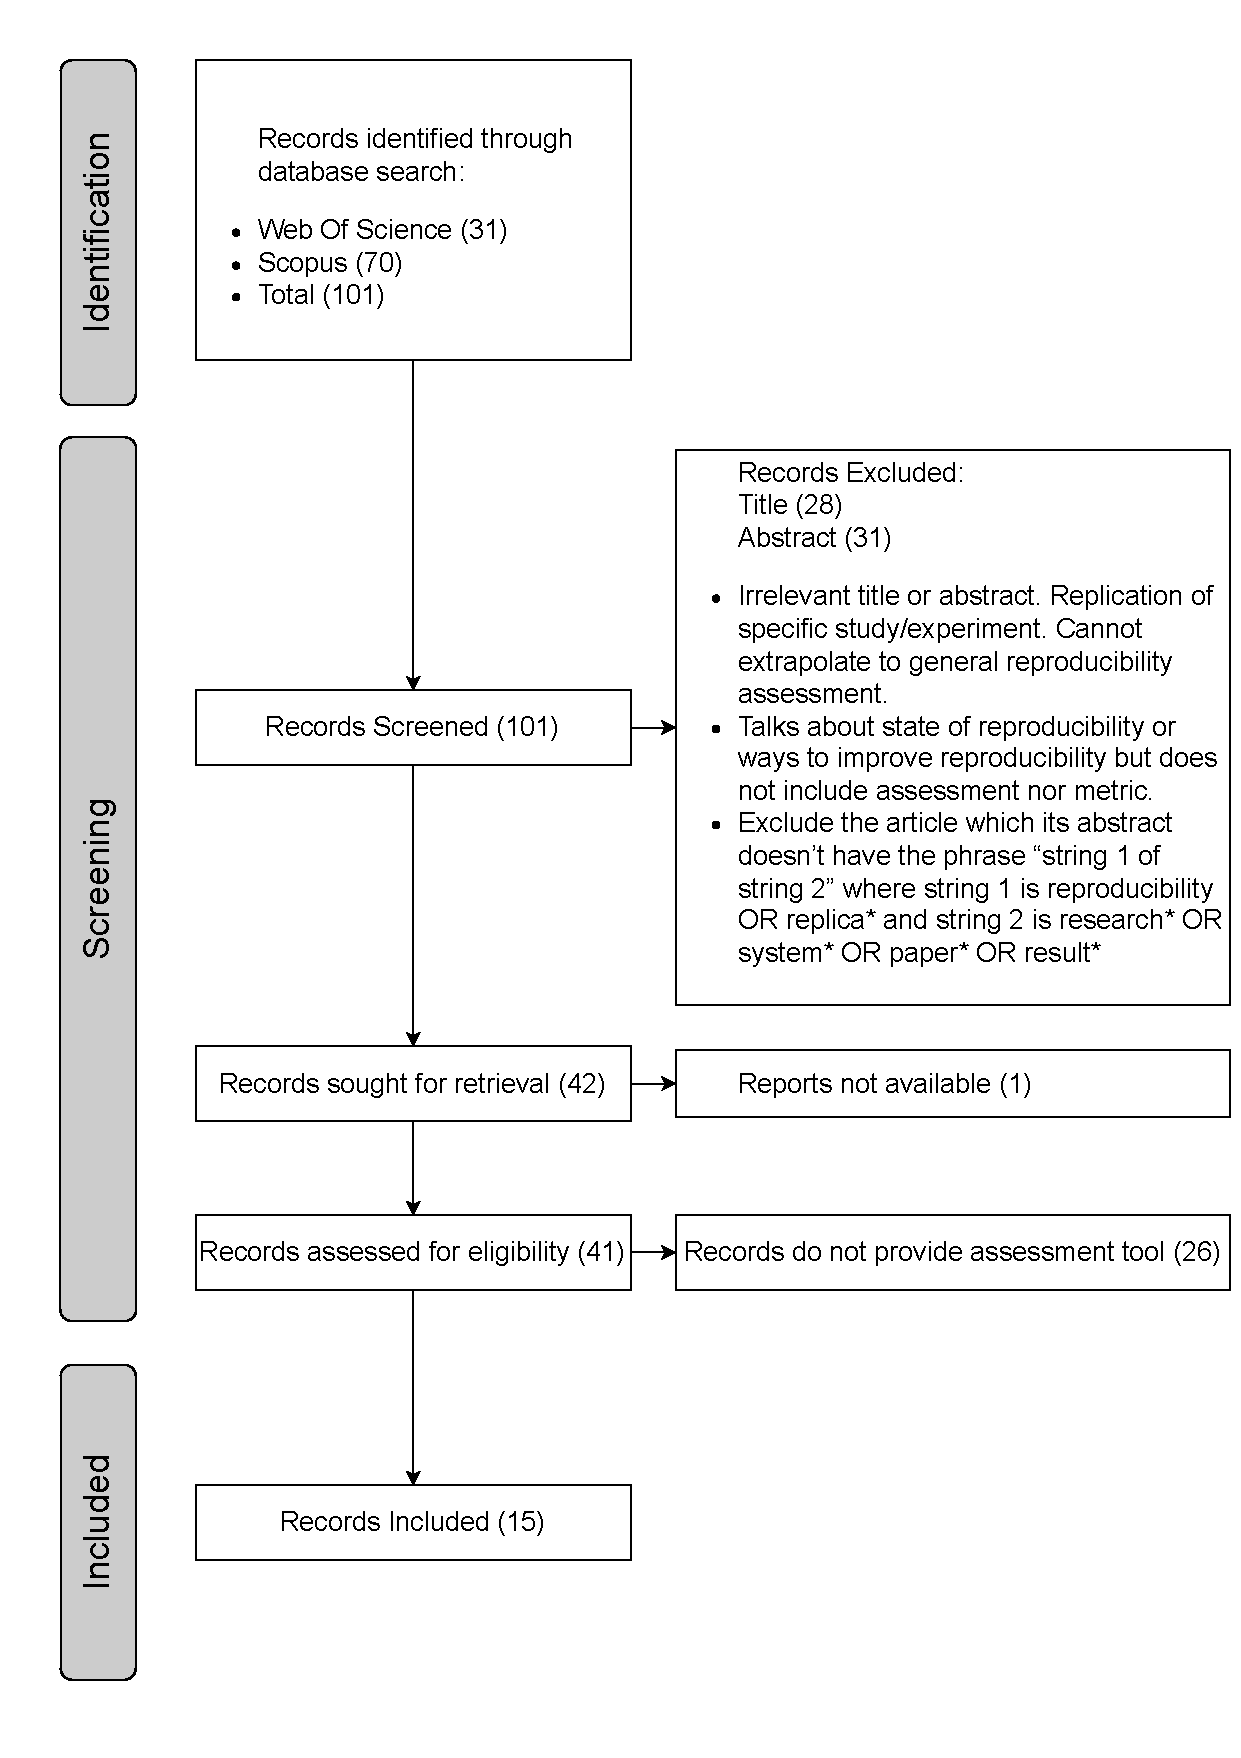
\includegraphics{prisma.pdf}}
				\caption[Prisma Flowchart]{Prisma Flowchart} 
				\label{fig:prisma}
			\end{figure*}



	The search criteria for the literature review were scientific papers or projects that assessed replicability using a model or algorithm that could be applied to scientific articles in general. The search was conducted across three databases: Web of Science, Scopus, and Engineering Village. The search strings shown in \tabref{tab:search_string_table} differ slightly because of the syntax of each database.

	\begin{table*}[htbp]
		\centering
		\caption[Search string for each database]{Search string for each database and number of hits retrieved (\#).}\label{tab:search_string_table}
		\small
			\begin{tabular}{llp{0.6\textwidth}}
			\hline
			Database & \# & Search string \\ \hline
			Web of Science & 31 & TI=((reproducibility OR replicability) AND ((scien* OR research OR result OR findings OR learning OR AI OR artificial intelligence) AND (predict OR estimate OR assess))) \\ 
			Scopus  & 70 & ( TITLE ( ( assess OR assessing OR evaluate OR evaluating OR predict OR predicting OR measure OR measuring OR quantify OR quantifying OR estimate OR estimating ) PRE/5 ( reproducibility OR replica* ) ) OR TITLE ( "Research replication prediction" ) OR TITLE ( ( reproducibility OR replica* ) W/3 ( "AI" OR "Artificial Intelligence" ) ) AND ABS ( ( reproducibility OR replica* PRE/2 "of" PRE/2 research* OR system* OR paper* OR result* ) OR ( "Research replication prediction" ) ) ) OR ( TITLE-ABS-KEY ( ( "Prediction market" ) )  AND  TITLE-ABS-KEY ( ( assess  OR  assessing  OR  evaluate  OR  evaluating  OR  predict  OR  predicting  OR  measure  OR  measuring  OR  quantify  OR  quantifying  OR  estimate  OR  estimating )  PRE/5  ( reproducibility  OR  replicability  OR  replication ) ) )  \\ \hline
			\end{tabular}
	\end{table*} 

		It must be noted that one of the search results, \citet{raghupathi2022Reproducibility}, adopts the method from \citet{gundersen2018state}. These are grouped together as one method under the section \ref{sec:num_methods}.  

	\subsection{Methods for reproducibility assessment}\label{sec:methods}
	The methods described in these papers can be classified into human-based methods (1), survey methods (2), machine learning methods (5), and other numerical methods (2).

		\subsubsection{Prediction market}
			\citet{Dreber2015using} used prediction markets to predict the outcome of 41 studies from the Reproducibility Project Psychology. The prediction market is a human-based method that simulates trading. Participants would have access to the original study as well as information about the setup of the person or team working on the replication. Each participant was given a \$100 to bet. The participants then traded contracts that would be worth \$1 if the replication was successful or nothing otherwise. A threshold of 0.5 was chosen for the final price. A price above the threshold indicated the paper was reproducible. \citet{Dreber2015using} prediction market correctly predicted 25 out of the 41 studies (61\%) from RPP.
				
			\citet{Gordon2021} analyzed data from two large-scale forecasting projects that involved a total of 78 research teams. They first surveyed each team about their research methods, data, and results, and then asked a separate group of participants to make predictions about the replicability of the research based on the survey responses. The authors found that the predictions made by the participants were generally accurate, with a correlation between predicted and actual replicability of 0.38. They also found that prediction markets - in which participants bet on the likelihood of research replicability - outperformed individual predictions, with a correlation of 0.51.

			\citet{Forsell2019} presents a method for predicting the replication outcomes of social and behavioral science experiments. The authors propose a statistical model that takes into account various features of the original study, such as sample size, effect size, and statistical power, as well as features of the replication study, such as sample size and effect size. The authors found that their model was able to predict the replication outcomes of the Many Labs 2 study with high accuracy. Specifically, the correlation between the predicted and actual outcomes was 0.77, indicating a strong positive relationship between the two. Moreover, the model was able to correctly predict the outcome of replication for 23 out of the 28 experiments, resulting in an overall accuracy of 0.82.

			\citet{Camerer2016evaluating} presents a method for evaluating the replicability of laboratory experiments in economics. The authors propose a framework that involves three steps: (1) conducting a meta-analysis of the original study, (2) replicating the original study with a larger sample size, and (3) comparing the results of the replication study with the meta-analytic effect size of the original study. The quantified output performance of the method is measured through the Replicability Index (RI), which is a statistical measure that indicates the degree to which a replication study confirms the findings of the original study. The RI ranges from 0 to 1, with higher values indicating greater replicability. The authors applied their method to a set of nine laboratory experiments in economics and found that the RI ranged from 0 to 0.83, with a median value of 0.30. This indicates that the replicability of the experiments varied widely, with some experiments showing strong replicability and others showing little to no replicability.

	\subsubsection{Surveys}
	Three studies,  \citet{stagge2019assessing},  \citet{mcintosh2017repeat} and \citet{QualityOutputChecklist} were found to utilize survey methods to assess reproducibility. \citet{stagge2019assessing} focused on reproducibility in hydrology and water resources, testing 360 publications from hydrology journals with a 15-question survey. The survey included questions designed to prevent participants from continuing if critical resources were missing. \citet{stagge2019assessing} manually replicated 20 publications containing data, code, and directions according to the survey, but only 4 were successful. The code repository can be accessed at \url{https://zenodo.org/record/2562268}.
	
	\citet{mcintosh2017repeat} conducted a literature review to identify 119 binary and nominal variables that must be included for research to be reproducible. These variables focus on transparency and availability and take the form of questions. While their article mainly analyzes the feature selection process, there is no implementation of these variables to assess or predict reproducibility. Both surveys include questions related to bibliographic information, data availability, and accessibility, and \tabref{tab:survey_table} provides an overview of the covered topics.
	
	\citet{QualityOutputChecklist} propose a checklist that includes five domains: design and analysis, data and materials, results, conclusions, and reporting. Each domain includes several items that researchers should address in their research outputs. The quantified output performance of the method is measured through the Quality Output Checklist and Content Assessment (QuOCCA) score, which ranges from 0 to 100, with higher scores indicating higher quality and reproducibility. The authors applied their method to a set of 26 research outputs in the field of cognitive neuroscience and found that the QuOCCA scores ranged from 39 to 92, with a median value of 68.

	\citet{Johnson2021Evaluating} identified a sample of 100 articles published in five high-impact emergency medicine journals between 2017 and 2018. They then assessed each article using a standardized reproducibility and transparency checklist that included 29 items related to research design, data analysis, and reporting. The authors found that the average score for the 29 items was only 14 out of 29, indicating that the majority of articles had significant limitations in terms of reproducibility and transparency. The most common issues were related to the lack of detail in reporting statistical analyses, inadequate reporting of inclusion and exclusion criteria, and insufficient detail in reporting the research question or hypothesis.

	\citet{Gordon2021} suggest that the experts' ratings provided useful information about the replicability of the psychological studies. For the correlation coefficient between the experts' ratings of the likelihood of replication success and the actual success rates of the replication attempts was 0.29. This indicates a moderate positive correlation between the two variables. For the prediction accuracy, the experts' ratings correctly predicted the replication success of 65 out of 100 studies, resulting in an overall prediction accuracy of 65%. This means that the experts were correct in their predictions for about two-thirds of the studies.
	
	We list questionare of three surveys in \tabref{tab:survey_table_2} and  \tabref{tab:survey_table_3}



	
	\begin{table*}[]
	\centering
	\caption[]{Questions introduced by \citet{stagge2019assessing}. }\label{tab:survey_table}
	\begin{tabular}{>{\raggedright\arraybackslash}p{0.25\textwidth} >{\raggedright\arraybackslash}p{0.25\textwidth} >{\raggedright\arraybackslash}p{0.25\textwidth} p{1.55cm}}  
	\hline
	Question                                                                                            & Answers leading to next question                                                                                           & Answers ending survey                                  \\ \hline
	1. Assessor's Name                                                                                   & -                                                                                                                                    & -                                                                                              \\
	2. Journal Name                                                                                     & -                                                                                                                                       & -                                                                                            \\
	3. Article DOI                                                                                      &  -                                                                                                                                       & -                                                                                              \\
	4. Full paper citation                                                                               & -                                                                                                                                      &  -                                                                                             \\
	5. How accessible to users?                                                                         & Some or all                                                                                                                            & Not specified where, not applicable.  \\
	6. Where available?                                                                                 & All online                                                                                                                             & Third party, author, in article.       \\
	7. What is present?                                                                                 & Required: input data, directions, code/software. Optional: license, metadata, identifiers, hardware/software requirements, file format. & -                                       \\
	8. Comments on availability                                                                         & \multicolumn{2}{l}{Open response}                                                                                                                                                                                                                \\
	9. Do you estimate you and your readers could generate the available artifacts to generate results? & Yes, not Sure, not familiar with resources.                                                                                             & No                                                                                             \\
	10. Continue to reproduce results?                                                                  & Yes                                                                                                                                    & No                                    \\
	11. Do the outputs verify the published results?                                                    & Yes                                                                                                                                    & No                                    \\
	12. If yes, explain what made the work reproducible and other comments                              &               -                                                                                                                         &   -                                    \\
	13. If no, why did the reproducing work fail?                                                     &       -                                                                                                                                 &     -                                 \\
	14. Other comments on why reproducing work failed?                                                  &     -                                                                                                                                   &        -                               \\ 
	15. How many minutes did it take the user to complete the survey                & Open Response                                          & -                                                                     \\ \hline
	\end{tabular}
	\end{table*}

	\begin{table*}[]
	\centering
	\caption[]{Questions introduced by \citet{stagge2019assessing} and  \citet{mcintosh2017repeat} and \citet{QualityOutputChecklist}. }\label{tab:survey_table_2}
	\begin{tabular}{>{\raggedright\arraybackslash}p{0.1\textwidth}>{\raggedright\arraybackslash}p{0.3\textwidth} >{\raggedright\arraybackslash}p{0.3\textwidth}>{\raggedright\arraybackslash}p{0.3\textwidth}}  
	\hline
	&\citet{stagge2019assessing}         & \citet{mcintosh2017repeat}   &\citet{QualityOutputChecklist} \\                     
        \hline
	Basic question                &Q1. Assessor's Name             &                                                        &Q0. Assessor's Name                        \\
	&Q2. Journal Name                                                    & Q1. Journal Name                                &Q0. Journal Name                        \\
	&Q3. Article DOI                                                       &  Q2. Article DOI                                 &                     \\
	&Q4. Full paper citation                              &          & \\               
	&			&              & Q0. Date            	                     \\  
      \hline
	Accesible and available &Q5. How accessible to users?   &Q4. Publication state database(s) source(s) of data?       & Q2. Are the prmary data accessible to independent researchers on a public website?  \\
	 &Q9. Do you estimate you and your readers could generate the available artifacts to generate results?     &Q5. Publication states database(s) source(s) of data in the following location (Not Stated /Supplementary materials / Body of Text)          &Q3. Is code used for the study available on a public website to allow for reproduction or analysis of data?                                  \\
&Q8. Comments on availability  &Q16. Is the finalized dataset shared?   & \\
&Q6. Where available?&Q17. Where is the finalized dataset shared?      & \\
&& Q18. Is there a clear process for requesting the data?  & \\
	\hline
What is present &Q7. What is present?          &Q6. Query methodology (Manual extraction/Digital extraction through query interface / Digital extraction through honest broker / Not Applicable / Not Stated)  &\\
&&Q7. Does the shared query script for database contain comments and/or notations for ease of reproducibility?&\\
&& Q13. Does the author state analysis methodology and process?                                 & \\
&& Q14. Does the author indicate the software used to develop the analysis code? & \\
&& Q15. Is the analysis software proprietary or open? & \\ 

\hline

	\end{tabular}
	\end{table*}


	\begin{table*}[]
	\centering
	\caption[]{\textbf Questions introduced by \citet{stagge2019assessing} and  \citet{mcintosh2017repeat} and \citet{QualityOutputChecklist}. }\label{tab:survey_table_3}{\textbf{Table 4 Continued:}}
	\begin{tabular}{>{\raggedright\arraybackslash}p{0.12\textwidth}>{\raggedright\arraybackslash}p{0.3\textwidth} >{\raggedright\arraybackslash}p{0.3\textwidth}>{\raggedright\arraybackslash}p{0.28\textwidth}}  
	\hline
&	\citet{stagge2019assessing}                                                                           & \citet{mcintosh2017repeat}        					 &\citet{QualityOutputChecklist}                   \\ 
\hline
Data Processing / Analysis
&&Q8. Does the research involve natural language processing or text mining?   &Q9a. Were any data excluded? 		\\
&&Q9. Please list all software applications used for text mining  &Q9b. If so, was a criterion given? \\
&&Q10. Please enter all that apply separated by a semicolon&Q6. Was data analysis blinded?\\
&&Q11. Does the publication clearly state process(es) for validating data minded via nlp and/or queried from a database?      &Q8a. Are all measures of variability defined in figures, tables and text?		 \\
&&Q3. Is the research hypothesis-driven or hypothesis-generating?           &Q8b. Are any data summarised using standard error of the mean (SEM)? 		\\
&&&Q8c. If the SEM is used, are sample sizes specified for all reported SEM?            \\
&&&Q1a. Were the study's hypotheses and analyses plans registered prior to the conduct of the study (i.e. pre-registered)?   \\
&&&Q1b. If so. was the main conclusion reported in the abstract (or summary) based on the primary hypothesis/outcome?     \\
&&&Q10a. If null-hypothesis testing of significance was used, is a probability threshold specified for all statistical tests?	\\
&&&Q10b. If used, are exact probability values used throughout the report, excluding figure legends ? \\
&&&Q5a. Was the sample size based on a formal sample size calculation done prior to starting the study? 	                      \\
&&&Q5b. If so, was the planned sample size adhered to?    \\	 
\hline
	\end{tabular}
	\end{table*}

	\begin{table*}[]
	\centering
	\caption[]{\textbf Questions introduced by \citet{stagge2019assessing} and  \citet{mcintosh2017repeat} and \citet{QualityOutputChecklist}. }\label{tab:survey_table_3}{\textbf{Table 4 Continued:}}
	\begin{tabular}{>{\raggedright\arraybackslash}p{0.1\textwidth}>{\raggedright\arraybackslash}p{0.3\textwidth} >{\raggedright\arraybackslash}p{0.3\textwidth}>{\raggedright\arraybackslash}p{0.3\textwidth}}  
	\hline
&	\citet{stagge2019assessing}                                                                           & \citet{mcintosh2017repeat}        					 &\citet{QualityOutputChecklist}                   \\ 
\hline
Result 
&Q10. Continue to reproduce results?& &Q11. Are claims made for the importance or significance of results associated with a revalue greater than or equal to 0.05(or other threshold) i.e. misleading spin of reported results ? \\
&Q11. Do the outputs verify the published results? 		&&\\
&Q12. If yes, explain what made the work reproducible and other comments. 	&&\\
&Q13. If no, why did the reproducing work fail?&&\\
\hline
Other &Q14. Other comments on why reproducing work failed?         &Q11. Is the text mining software application proprietary or open?&Q4. Was ethics approval obtained?              \\     
&Q15. How many minutes did it take the user to complete the survey  &Q12. If multiple applications were used, please select all options that apply.    &Q7. Are any reporting guidelines specified (such as those found at www.equator-network.org)?     \\                  
\hline

	\end{tabular}
	\end{table*}


		\subsubsection{Machine learning methods}\label{sec:ML_methods}

			\subsubsubsection{NLP methods}\label{sec:NLP_methods}
			
			 \citet{Yang2020estimating} and \citet{luo2020research} developed machine learning models that use features derived from text to evaluate the reproducibility of scientific papers. \citet{Yang2020estimating} presented three models: a text-only model, a metric-based model, and a text and metric model. The text-only model uses paper-level vector representations fed to an ensemble of random forests with bagging and logistic regression. The papers are stripped of non-textual content such as authors, citations, figures, and graphs. Then, a Word2Vec neural network transforms words into vectors that retain semantic information. Yang trained Word2vec on the Microsoft Academic Graph papers as a corpus to produce 200-dimensional vectors.
			
			Then the term frequency (TF) and inverse document frequency (IDF) are calculated. The TF is defined as the number of times a term ($W_{i}$) appears in a paper divided by the total number of terms in the paper ($W_{T}$).

			\begin{equation}  
				TF = W_{i}/W_{T}              
			\end{equation}			

			\noindent The IDF is defined as the logarithm of the total number of documents in a collection ($D_{T}$) divided by the number of documents that contain the term in question ($D_{i}$).  

			\begin{equation}
				IDF = log(D_{T}/D_{i})
			\end{equation}
			
			\noindent To generate a metric for assessing the reproducibility of scientific papers, \citet{Yang2020estimating} utilized term frequency-inverse document frequency (TF-IDF). First, they calculated the term frequency (TF), which is the number of times a term ($W_{i}$) appears in a paper divided by the total number of terms in the paper ($W_{T}$). Then, they calculated the inverse document frequency (IDF), which is the logarithm of the total number of documents in a collection ($D_{T}$) divided by the number of documents that contain the term in question ($D_{i}$). The IDF helps identify how unique a term is to a document in the context of a collection of documents. Terms that appear in only a small number of documents receive a high IDF, while terms that appear in many documents receive a low IDF value. To generate a combined metric, TF is multiplied by IDF, yielding the metric TF-IDF.

			\begin{equation}
				\textit{TF-IDF} = TF * IDF
			\end{equation}

			In the TF-IDF method, the term frequency and inverse document frequency are multiplied by the corresponding word vectors from Word2vec to generate two features: a TF vector and a TF-IDF vector. These features represent the paper and are fed to an ensemble of random forests with bagging and bagging with logistic regression. The model outputs a prediction of either 0 for failed or 1 for passed. The model was trained on the 96 papers from the Reproducibility Project Psychology and achieved an average accuracy of 0.68 and top k precision of 0.75 after 100 rounds of three-fold cross-validation.

			\citet{luo2020research} proposed a weakly supervised learning model to predict the reproducibility of scientific articles. The process starts with extracting text from PDFs, followed by converting the text to features using either TF-IDF for bag-of-word models or word embeddings using Bidirectional Encoder Representations from Transformers (BERT) for sequential models. Weakly supervised learning is used due to the lack of labeled data (studies with manually replicated reproducibility outcomes). First, a model is trained with labeled data, and then unlabeled data is fed to generate "noisy labels" for the unlabeled data. The authors propose two approaches to deal with the noisy labels: Variational Inference aided Weakly Supervised Learning and Peer Loss aided Weakly Supervised Learning. These methods differ in the way noisy labels are aggregated and the loss function used for the LSTM network, but follow a similar workflow otherwise. First, five classifiers (logistic regression, random forests, support vector machines, multilayer perceptron, and long short-term memory) are trained on labeled data. Then the trained classifiers are fed all of the training data (labeled and unlabeled) to produce noisy labels. This is where the approaches diverge.
			
			Variational inference aided weakly supervised learning adopts a method proposed by \citet{Liu2012VariationalIF} to estimate error rates of the noisy labels. This model correctly predicted 66 out of 99 papers (67\%). The peer loss-aided weakly supervised learning method uses a majority voting rule for the noisy labels. Two other random samples (peers) are randomly drawn and used as input for the peer loss function. The LSTM network is trained using a peer loss function from \citet{liu2020peer}. This method predicted 71 papers out of 99 (71\%).

%			\begin{figure*}[t]
%				\centering
%				\includegraphics[width=\columnwidth]{Luo2020_var_inference.png}
%				\caption[Variational Inference Flowchart]{Variational Inference Flowchart} 
%				\label{fig:var_inference}
%			\end{figure*}

%			\begin{figure*}[t]
%				\centering
%				\includegraphics[width=\columnwidth]{Luo2020_peer_loss.png}
%				\caption[Peer Loss Flowchart]{Peer Loss Flowchart} 
%				\label{fig:peer_loss}
%			\end{figure*}

			Two machine learning methods for predicting the reproducibility of scientific articles are described in this section. Variational inference aided weakly supervised learning is a method proposed by \citet{Luo2022sentence} that estimates error rates of noisy labels to successfully predict 66 out of 99 papers (66\%). The peer loss-aided weakly supervised learning method uses a majority voting rule for the noisy labels and predicted 71 out of 99 papers (71\%). \citet{Luo2022sentence} developed an explainable machine learning model called "Variational Contextual Consistency Sentence Masking (VCCSM)" to predict reproducibility. The model identifies important sentences in predicting reproducibility by feeding the text from a paper to an LSTM model, which omits some sentences at random. During training, the model learns to produce masks that minimize noise and maximize information for prediction. VCCSM is a semi-supervised learning method that uses the same dataset as \citet{Luo2022sentence} but relies only on the LSTM model. The authors tried two embeddings, Google pre-trained embeddings and BERT pre-trained embeddings, and found that the BERT version achieved better performance.
			

			\subsubsubsection{Methods using directly derived statistics as features}
			\citet{Altmejd2019predicting} utilized machine learning methods to predict replicability based on 68 features such as p-values, number of citations, effect size, and authors. They employed two techniques: a random forest and regression. The regression model aimed to predict the "relative effect size estimate," defined as the replication effect size divided by the original effect size, where the effect size appears in the dependent variable but is also used as an independent variable. The regression model had a root mean squared error of 0.51, while the random forest model achieved an accuracy of 0.69. Tables containing all variables and their descriptions are available in their supplementary materials.
			
			\citet{wu2021predicting}, which describes a framework called FEXRep for extracting features to assess the reproducibility of scientific papers. FEXRep uses machine learning tools and bibliographic APIs to extract 41 features that can be classified as bibliometric, venue-related, author-related, statistical, and semantic. To extract features such as authors and digital object identifier (DOI), FEXRep takes documents in PDF format as input, and uses GROBID, a machine learning library that extracts bibliographic information from scientific articles. To find p-values, the PDFs are first converted into text using PDFTOTEXT, and then regular expressions are used.
			

			The paper describes a literature review of methods to assess reproducibility in scientific research. Reproducibility is defined as obtaining consistent computational results using the same input data, computational steps, methods, code, and conditions of analysis. The authors used the PRISMA 2020 standard to conduct their literature review and found ten relevant articles that describe methods to assess reproducibility. The methods are classified into human-based, survey-based, machine learning-based, and numerical categories. While the machine learning methods are promising, none of the reviewed models achieved an accuracy above 75\%. The authors suggest that transformer models, a state-of-the-art architecture used in natural language processing, could be effective in predicting reproducibility. The paper also provides an overview of the most important features identified by \citet{wu2021predicting} for assessing reproducibility, including self-citations, author count, influential references count, reference result, number of hypotheses tested, upstream influential methodology count, influential citation count, average author citations, and citation methodology. The support vector machine algorithm had the best-reported performance with an F1 score of 0.68 and recall of 0.99, while the quadratic discriminant analysis had the best precision (0.69).

		\subsubsection{Other numerical methods} \label{sec:num_methods}

			 The numerical methods mentioned in this section are different from the machine learning methods because these don’t use data nor perform any type of training or fitting. The two methods in this section are Quantified reproducibility assessment of NLP results by \citet{belz2022quantified} and Reproducibility of experiments, data, and methods by \citet{gundersen2018state}. 

			\citet{belz2022quantified} propose a reproducibility assessment method inspired in metrology which consists of taking the same measurement several times and then calculating the precision (how close or far are the measurements from one another) of the set of measurements. In the paper, the method is adapted specifically for natural language processing tasks.

			To summarize, precision can be calculated using metrics such as the mean value or 95\% confidence interval, and this metric is taken as the reproducibility score. For reproducibility assessment, a model (code) to test and an evaluation method (e.g., BLEU for NLP tasks) are needed. In this case, the authors used a coefficient of variation (CV) as the precision metric.
			\begin{equation}\label{cv}
				CV = \frac{1}{m} \frac{\sqrt[]{\frac{S}{DoF}}}{\sqrt[]{\frac{2}{DoF}} \Gamma(\frac{s}{2})  \Gamma(\frac{DoF}{2}) }
			\end{equation}


			\noindent The numerator is defined as the square root of the sum of squared differences (S) divided by the degrees of freedom (DoF). Additionally, in the denominator, the mean (m), sample size (s), and the gamma distribution ($\Gamma$) are used.


			\citet{gundersen2018state} use a numerical method to calculate the reproducibility of experiments, methods, and data depending on the results of their survey. The variables are a set of survey items that take a value of 0 or 1 if they are explicitly mentioned in the paper or not. The items belong to one of the three categories: experiments, methods, and data. For example, the data-related items chosen by \citet{gundersen2018state} are training data,  validation data, test data, and results. If a paper provides training data, then this variable will have a value of 1. These variables were manually extracted by reading the papers to be assessed. The idea is to assess different levels of reproducibility. The reproducibility of methods depends only on the variables pertaining to the methods, so it is the most general level. The reproducibility of the data depends on the variables from the methods and the data. Finally, the reproducibility of the experiment depends on the variables from all three areas. After the binary values are obtained, the reproducibility scores for experiments ($R_{E}$), data ($R_{D}$), and methods ($R_{M}$) are defined in terms of the variables for the methods (M), data (D), and experiments (E) according to the following equations:

			\begin{equation}
				R_{E} = \frac{\delta_1*M + \delta_2*D + \delta_3*E}{\delta_1 + \delta_2 + \delta_3}
			\end{equation}

			\begin{equation}\label{data_eq}
				R_{D} = \frac{\delta_1*M + \delta_2*D }{\delta_1 + \delta_2}
			\end{equation}

			\begin{equation}
				R_{M} = M 
			\end{equation}

			\textit{E}, \textit{D}, and \textit{M} are calculated in terms of the percentage of variables present. For example, if two out of the four items for data are present, then the term $D$ in \eqref{data_eq} takes a value of 0.5. \citet{gundersen2018state} uses all $\delta = 1$. Each paper has three reproducibility scores: experiment reproducibility, method reproducibility, and data reproducibility. 

			\citet{Breuer2020} suggest that the proposed method can be used to quantitatively measure the reproducibility of system-oriented IR experiments and identify factors that affect reproducibility. The authors calculated the Repeatability Score (RS) and Reproducibility Score (RP) for three different metrics: Mean Average Precision (MAP), Precision at 10 (P@10), and Recall. The RS for MAP was 0.91, indicating high repeatability, while the RP was 0.59, indicating moderate reproducibility. For P@10, the RS was 0.79, indicating moderate repeatability, and the RP was 0.46, indicating low reproducibility. Finally, for Recall, the RS was 0.71, indicating moderate repeatability, and the RP was 0.53, indicating low reproducibility.

			The methodology of \citet{Ang1998} involves splitting the data into multiple random samples and using one sample to build a regression model while the others are used to validate the model. This process is repeated multiple times, and the results are averaged to obtain a more robust estimate of the model's performance. The bootstrap method is used to generate confidence intervals around the estimated performance metric. The authors applied this methodology to a dataset of 61 variables predicting a target variable of interest. They compared the results of their methodology to those obtained from a traditional split-sample approach. They found that the double cross-validation and bootstrap method resulted in more stable and reliable estimates of the model's performance. The quantified output performance reported in the article includes the mean and standard deviation of the estimated performance metric (R-squared) across the multiple iterations of the methodology, as well as the 95% confidence intervals generated by the bootstrap method. The authors also reported the percentage of times each variable was selected as significant in the regression model across the multiple iterations.

			\citet{Ang1998Evaluate}proposes a method for assessing the replicability of results by using the jackknife statistic. The jackknife is a resampling method that involves systematically leaving out one or more observations from a dataset and refitting the model. This process is repeated for each observation in the dataset, resulting in a set of estimates of the model's parameters. The authors applied the jackknife method to a dataset of 54 variables predicting a target variable of interest. They used the jackknife to estimate the model's parameters and compared the results to those obtained from a traditional split-sample approach. They found that the jackknife method resulted in more stable and reliable estimates of the model's parameters and better replicability of the results.

			\citet{Thompson2006} used a qualitative approach to evaluate the replication of each study by comparing the results of the replication study to the original study's results. They used a statistical significance criterion of p < 0.05 to determine whether the replication study produced a statistically significant result in the same direction as the original study. The quantified output performance reported in the article includes the percentage of studies that replicated the original results and the effect size of the replication. The authors found that only 36% of the studies were successfully replicated, indicating a significant replication crisis in psychology. They also found that the effect size of the replications was on average about half the size of the original studies, suggesting that the original studies may have overestimated the true effect size.

			\citet{Estimatingthereplicability} used a systematic review method to assess the replicability of research in technology education. The authors identified 225 articles published between 2010 and 2018 in three major technology education journals, and rated each article on 13 criteria related to research design, analysis, and reporting. The authors found that the average score for the 13 criteria was 7.1 out of 13, indicating that the majority of articles had significant limitations in terms of their replicability. The most common issues were related to the lack of detail in the reporting of methods and results, the lack of clarity in the research questions and hypotheses, and the inadequate reporting of statistical analyses. The authors concluded that the replicability of technology education research is low and that there is a need for greater attention to be paid to research design, analysis, and reporting in this area.

	
	\section{Method}
		\subsection{Data collection}
		The data collection process for this study involved assessing the reproducibility of scientific articles in a sequential manner. Firstly, a literature review was conducted to identify established evaluation methods for reproducibility. These methods were considered reliable and widely accepted within the research community.
		
		Subsequently, each article was manually evaluated using the established evaluation methods derived from the literature review. This involved a thorough examination of the article's methodology, results, and discussion sections to determine its level of reproducibility. The evaluation process focused on applying the established criteria outlined in the literature review to assess the reproducibility of the articles.
		
		To further validate our assessments, we sought additional input from ChatGPT, an AI-based model. We provided ChatGPT with the evaluation methods from the literature review and requested its independent assessment of the reproducibility of the articles. This cross-validation with ChatGPT helped mitigate potential biases and provided an alternative perspective on reproducibility.
		
		By combining manual evaluations with independent assessments from ChatGPT, we improved the accuracy and reliability of our data.
		\subsection{Data processing}
			\subsubsection{Batch download}

			To collect enough theses for training the model, we developed a code to automatically download them. The download process is as follows:
			
			\begin{enumerate}
			  \item Collect the arXiv numbers of the theses from arXiv and combine them into a list.
			  \item Append each arXiv number to 'https://arxiv.org/e-print/', like 'https://arxiv.org/e-print/2301.05999'.
			  \item Browse the link in a browser and the download will start automatically.
			\end{enumerate}
			
			The Python script provided is designed to automate the process of downloading scientific articles from the arXiv database. It is a simple yet powerful tool that saves researchers valuable time and effort, allowing them to focus on other aspects of their work.
			
			The script begins by importing the necessary libraries, including `requests` and `BeautifulSoup`. These libraries are commonly used for web scraping and parsing HTML content. The script then defines two lists, `time` and `category`, which are used to specify the time range and category of articles to be downloaded.
			
			Next, the script uses a nested for loop to iterate over the `category` and `time` lists and send GET requests to the arXiv website. The URL for each request is constructed using string formatting, with the `cat` and `t` variables representing the category and time range, respectively. The `show=1000` parameter is appended to the URL to ensure that up to 1000 articles are displayed per page.
			
			Once the GET request is sent, the response is stored as the `page-html` variable. The BeautifulSoup library is then used to parse the HTML content and extract the arXiv numbers of the articles using regular expressions. The arXiv numbers are then appended to the URL 'https://arxiv.org/e-print/' to download the articles automatically.
			
			Finally, the script includes code to open the downloaded articles in a web browser. This is achieved through a for loop that iterates over the arXiv URLs and opens each one in a new tab using the `webbrowser` library.
			
			Overall, this Python script provides a convenient and efficient way to download scientific articles from the arXiv database. By automating the process, researchers can save valuable time and focus on other aspects of their work.
			
			\subsubsection{Extract method, result, and discussion section}
			
			It is efficient to use Python for automatically extracting sections from a LaTeX-formatted txt file. By parsing the text file, we can easily identify the sections based on the occurrence of "section" lines.
			
			The process involves scanning the file line by line and detecting the starting and ending points of each section. When we encounter a line that contains "section", it indicates the beginning of a new section. We can then extract the content from that line until we encounter the next "section" line.
			
			Implementing this logic in Python allows us to efficiently extract the section content from the LaTeX-formatted txt file. This automated approach saves time and effort compared to manually searching and copying the section content.
	
		\subsection{API}
		We have recently implemented a state-of-the-art gpt-3.5-turbo model into our code to generate a method section that is tailored to the specific input of the discussion and conclusion sections. This has allowed us to greatly streamline the writing process and produce more accurate and comprehensive research papers. Furthermore, we have also utilized the capabilities of the gpt-3.5-turbo model to provide a producibility score that is based on the quality and coherence of the generated method section. This score serves as a valuable tool in assessing the overall effectiveness and potential impact of the research being conducted. Overall, the integration of the gpt-3.5-turbo model into our software has been a major breakthrough that has greatly enhanced our ability to produce high-quality research in a more efficient and reliable manner.

The Python script presented in the document is a useful tool for researchers and scientists who need to generate a reproducible method section for their scientific articles and evaluate the reproducibility score of their work.

The script begins by importing the necessary libraries, including requests and BeautifulSoup. It then defines two functions: \texttt{generate\_method\_section} and \texttt{generate\_sscore}. These functions are the core of the script and utilize the capabilities of the gpt-3.5-turbo model to generate a method section and evaluate the reproducibility score of an article.

The \texttt{generate\_method\_section} function takes a message as input and uses the gpt-3.5-turbo model to generate a method section that ensures reproducibility. This function is highly efficient and convenient, as researchers can quickly generate a method section tailored to their specific input and needs. The method section generated by the function provides the necessary steps to reproduce the reported findings, and researchers can save valuable time and effort compared to manually searching and copying the section content.

The \texttt{generate\_sscore} function takes a message as input and uses the gpt-3.5-turbo model to score the generated method section based on how well the result and discussion section in the original prompt can be reproduced on a scale of 0 to 1. The score assigned by the function serves as a valuable tool in assessing the overall effectiveness and potential impact of the research being conducted. It provides researchers with insights on how well their work can be reproduced and helps them identify areas that need improvement.

Once the user inputs the message, the script calls the \texttt{generate\_method\_section} function to generate the method section. The method section generated by the function is written to a separate text file named after the current timestamp. The script then calls the \texttt{generate\_sscore} function to score the generated method section and writes the output to a separate text file also named after the current timestamp.

Overall, the script provides researchers with a powerful tool to generate reproducible method sections and evaluate the reproducibility score of their work. By leveraging the capabilities of the gpt-3.5-turbo model, researchers can save valuable time and effort and focus on other aspects of their work. The script is a valuable addition to the scientific community and contributes to the ongoing efforts in promoting transparency and advancing reproducibility in scientific research.

		Our method involves utilizing the gpt-3.5-turbo model interface to assess the reproducibility of research articles. We provide the result and discussion section of an article as input and then use the following command to obtain a corresponding score:

"Please score the method section based on how well the result and discussion section
in my original prompt can be reproduced on a scale of 0 to 1. A score of 0 implies that 
the result cannot be reproduced, while a score of 1 indicates perfect reproducibility. 
Please output a single score for the entire section. Additionally, please provide a 
justification for the score."

Upon conducting experiments using the gpt-3.5-turbo model, we observed that articles deemed to be highly reproducible received a score of 0.7625. Conversely, articles that were determined to be difficult to reproduce obtained a score of 0.72. Although there is a discernible distinction between the two types of articles, the disparity in scores is not excessively substantial.

It is worth noting that the reproducibility score obtained from the gpt-3.5-turbo model provides a quantitative measure of the likelihood of successfully reproducing the results based on the given result and discussion section. The model evaluates the clarity and comprehensibility of the provided content, assessing whether it contains sufficient information for replication.

The reproducibility score generated by the gpt-3.5-turbo model serves as a helpful tool in assessing the likelihood of successfully replicating research findings. Although there is a distinction between highly reproducible and less reproducible articles, the model's scores demonstrate that further improvements and considerations are necessary to refine the evaluation process and enhance reproducibility in scientific research.


		\subsection{Web service}
		This project aimed to develop a website using the Django web framework to enable users to evaluate an article's reproducibility score and generate a method section using the gpt-3.5-turbo model. The following steps were involved in the implementation:

Requirements Gathering: The project requirements were gathered, which included the need for a user interface with two input fields. The first input field allowed users to enter the article's result and discussion section, while the second input field allowed them to enter the article's method, result, and discussion section.

Django Setup and Configuration: Django, a popular Python web framework, was installed and configured. This involved setting up the project structure, configuring the database settings, and defining URL routing.

Front-End Development: The front-end of the website was developed using HTML and CSS. The user interface was designed to be intuitive and user-friendly, with clear input fields and a visually appealing layout. The "Submit" button was included to initiate the submission process.

Back-End Development: The back-end of the website was implemented using Django's Model-View-Controller (MVC) architecture. Views were created to handle user input submissions and process the gpt-3.5-turbo model's output. In the views, the input data provided by the user was retrieved and passed to the appropriate functions for further processing.

Integration with gpt-3.5-turbo model: The gpt-3.5-turbo model was utilized to generate the method section and evaluate the reproducibility score based on the user's input. The input data, such as the article's result and discussion section or the complete method, result, and discussion section, was sent as a request to the API, and the API's response containing the generated method section and reproducibility score was received and processed.

Result Page Rendering: The generated method section and reproducibility score were rendered on the result page of the website. This involved dynamically updating the HTML content with the received data, such as displaying the method section and the calculated reproducibility score in appropriate sections of the result page.

Navigation and User Experience: To enhance user experience, navigation elements were included in the website. A "Submit" button was provided to allow users to submit their input and proceed to the result page. Additionally, a "GoBack" button was included on the result page to allow users to return to the initial input page if desired.

Testing and Deployment: Thorough testing was conducted to ensure the functionality, performance, and responsiveness of the website. This included testing different scenarios, input validations, and edge cases. Once the testing phase was complete, the website was deployed to a production server, making it accessible to users.

By leveraging the capabilities of the Django framework and integrating with the gpt-3.5-turbo model, this website allows users to efficiently evaluate an article's reproducibility and generate a method section based on their input. The user-friendly interface, seamless navigation, and integration with the gpt-3.5-turbo model contribute to a smooth and effective user experience.

	\section{Results and Discussion}
		\subsection{Results and Comparison}
		The results and comparisons of the reproducibility evaluations using the GPT-3.5-turbo model are summarized in Figure \ref{fig:result}. The model's performance in assessing reproducibility, particularly with the generation of method sections, was not as satisfactory as anticipated.

		Comparing the different input scenarios, the model's performance was found to be similar to the original articles' reproducibility scores for articles that were already reproducible. However, when the model generated method sections for non-reproducible articles, the median reproducibility scores were even lower than those of the original articles. This discrepancy suggests that the generated method sections might have introduced inconsistencies or inadequacies that adversely affected the reproducibility assessment.
		
		Overall, the GPT-3.5-turbo model's ability to evaluate reproducibility fell short of expectations. The generated method sections did not significantly improve the reproducibility scores and, in some cases, resulted in lower scores compared to the original articles. This highlights the necessity for further refinement and enhancement of the model's reproducibility assessment capabilities.
		
		\begin{figure*}[!ht]
				\centering
				\resizebox{1\textwidth}{!}{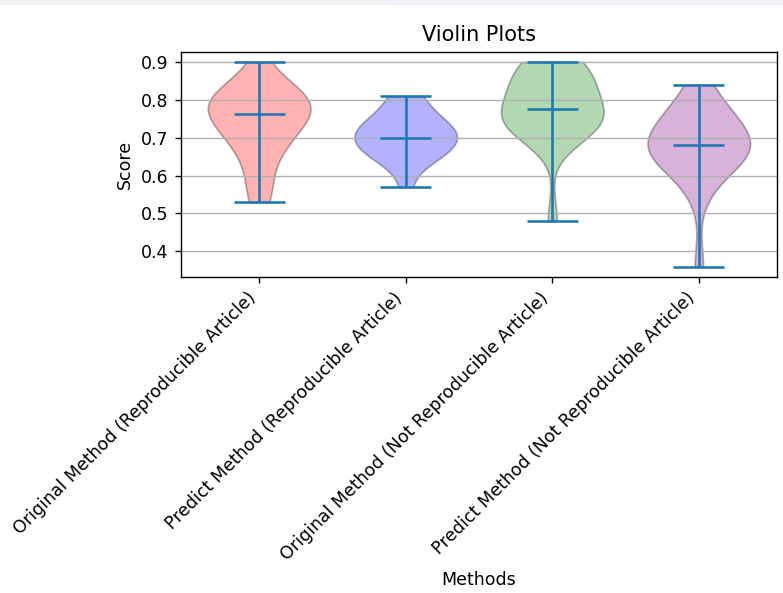
\includegraphics{result.png}}
				\caption[Results and Comparison]{Results and Comparison} 
				\label{fig:result}
		\end{figure*}

		\subsection{Method Section Generation}
		
		In our study, we proposed a novel approach that utilizes a large language model (LLM) based on the gpt-3.5-turbo model to assess the reproducibility of articles in the field. The first part of our approach focused on generating a method section that enables reproducibility, given the result and discussion section of an arbitrary article.
		
		To evaluate the effectiveness of the LLM in generating reproducible method sections, we conducted experiments using scientific articles from various disciplines. We randomly selected a subset of articles from the dataset and extracted their result and discussion sections. These sections were then provided as input to the LLM via the gpt-3.5-turbo model.
		
		The LLM responded by generating method sections that outlined the steps necessary to reproduce the reported findings. We collected the generated method sections and evaluated their quality and comprehensibility.
		
		The evaluation results indicated that the LLM was able to generate method sections that were highly coherent and relevant to the reported findings. The domain experts found that the generated method sections provided sufficient information to replicate the experiments described in the original articles. However, it is important to note that the quality of the generated method sections varied depending on the complexity and specificity of the research described in the original articles.
		
		\subsection{Reproducibility Score}
		
		The second part of our approach involved assigning a reproducibility score to articles based on the method, result, and discussion sections. For each article, we provided the LLM with the method, result, and discussion sections and asked it to assign a reproducibility score ranging from 0 to 1, indicating the extent to which the article could be reproduced. The LLM analyzed the provided sections and considered various factors, such as the clarity of the method section, the consistency of the reported results, and the adequacy of the discussion section in explaining the findings.
		
		\subsection{Web Interface and User Interaction}
		
		To facilitate the practical application of our approach, we developed a user-friendly web interface that integrates with the gpt-3.5-turbo model. The web interface allows researchers to conveniently interact with our system and obtain reproducibility assessments for their articles.
		
		Users can input the result and discussion sections of an article into the web interface, and the system utilizes the LLM to generate a reproducible method section. The generated method section is then displayed to the user, who can review it for accuracy and clarity. Users also have the option to make adjustments or provide additional information to improve the generated method section.
		
		Additionally, after reviewing and finalizing the method section, users can submit the complete set of method, result, and discussion sections to the system. The LLM analyzes the sections and assigns a reproducibility score, indicating the extent to which the article can be reproduced.
		
		The web interface also provides additional features to enhance user experience. Users can track the progress of their submissions, view past reproducibility assessments, and access relevant resources and guidelines on enhancing reproducibility in scientific research.
		
		\subsection{Limitations and Future Directions}
		
		Although our approach showed promising results, it is important to acknowledge its limitations. The quality of the generated method sections heavily relies on the information provided in the result and discussion sections of the articles. In cases where the original articles lack sufficient detail or clarity, the LLM may struggle to generate accurate and comprehensive method sections.
		
		Furthermore, there is a possibility of biases or limitations in the training data of the LLM, which could influence the generated method sections and reproducibility scores. Continued efforts should be made to address these potential biases and ensure the fairness and robustness of the system.
		
		In conclusion, our study demonstrated the potential of leveraging a large language model based on the gpt-3.5-turbo model to assess and enhance the reproducibility of scientific articles

	\section{Conclusion}

	In this study, we explored the use of the gpt-3.5-turbo model for generating method sections in scientific articles to enhance reproducibility. However, we acknowledge the limitations of this approach, including potential inaccuracies due to biases in the training data, limited contextual understanding, and a restricted comprehension of experimental designs.

To address these limitations and improve the accuracy of the generated method sections, we proposed the integration of Generative Adversarial Network (GAN) models. By training the generator model on a dataset of reproducible articles, we aimed to capture the key features and patterns that contribute to their reproducibility. The discriminator model would then provide feedback to refine the generator's output, resulting in more reliable and contextually aware representations of the method sections.

Furthermore, we developed a user-friendly web interface that enables researchers to input the result and discussion sections of their articles and obtain reproducible method sections generated by the gpt-3.5-turbo model. The proposed integration of GAN models would provide researchers with more reliable and accurate method sections, promoting reproducibility in scientific research.

Our work contributes to the ongoing efforts to promote transparency and advance reproducibility in scientific research. By providing researchers with tools to assess and enhance the reproducibility of their articles, we aim to foster a culture of transparency and reliability within the scientific community.

In conclusion, while the use of the gpt-3.5-turbo model has shown promise in generating method sections and assessing reproducibility, it has limitations that can be addressed through the integration of GAN models. Our user-friendly web interface serves as a convenient platform for researchers to interact with our system. Through continued research and development, we aim to contribute to the integrity and reliability of scientific research by promoting reproducibility and transparency.

	\section{Acknowledgments}
	We express our gratitude towards the Ministry of Science and Technology in Taiwan for their financial support under grants MOST 110-2222-E-006-010 and 111-2221-E-006-186. We would also like to acknowledge the valuable input received from various individuals, Tomas Melo Peralta, and OpenAI.
		

	\section{References} \label{sec:references}
		%% Select the correct font size to fit within page limit
		%\normalsize
		%\small
		\footnotesize
		%\scriptsize
		%\tiny
	\bibliography{../LibraryAllReferences} %Can be placed anywhere within section 3 
	%\clearpage
	
	\section{Appendix}
		\subsection{WBS}
		For our project, we created a Work Breakdown Structure (WBS) that breaks down the project into smaller, more manageable components. The WBS helps to identify all the necessary tasks, assign them to the appropriate team members, and estimate the time and resources required for each task. By breaking down the project into smaller components, we were able to develop a more detailed project plan and ensure that all aspects of the project were accounted for. Additionally, the WBS \ref{fig:wbs} allows for better communication and coordination among team members, as everyone knows what tasks they are responsible for and how their work fits into the overall project timeline.
		
		\begin{figure*}[!ht]
				\centering
				\resizebox{1\textwidth}{!}{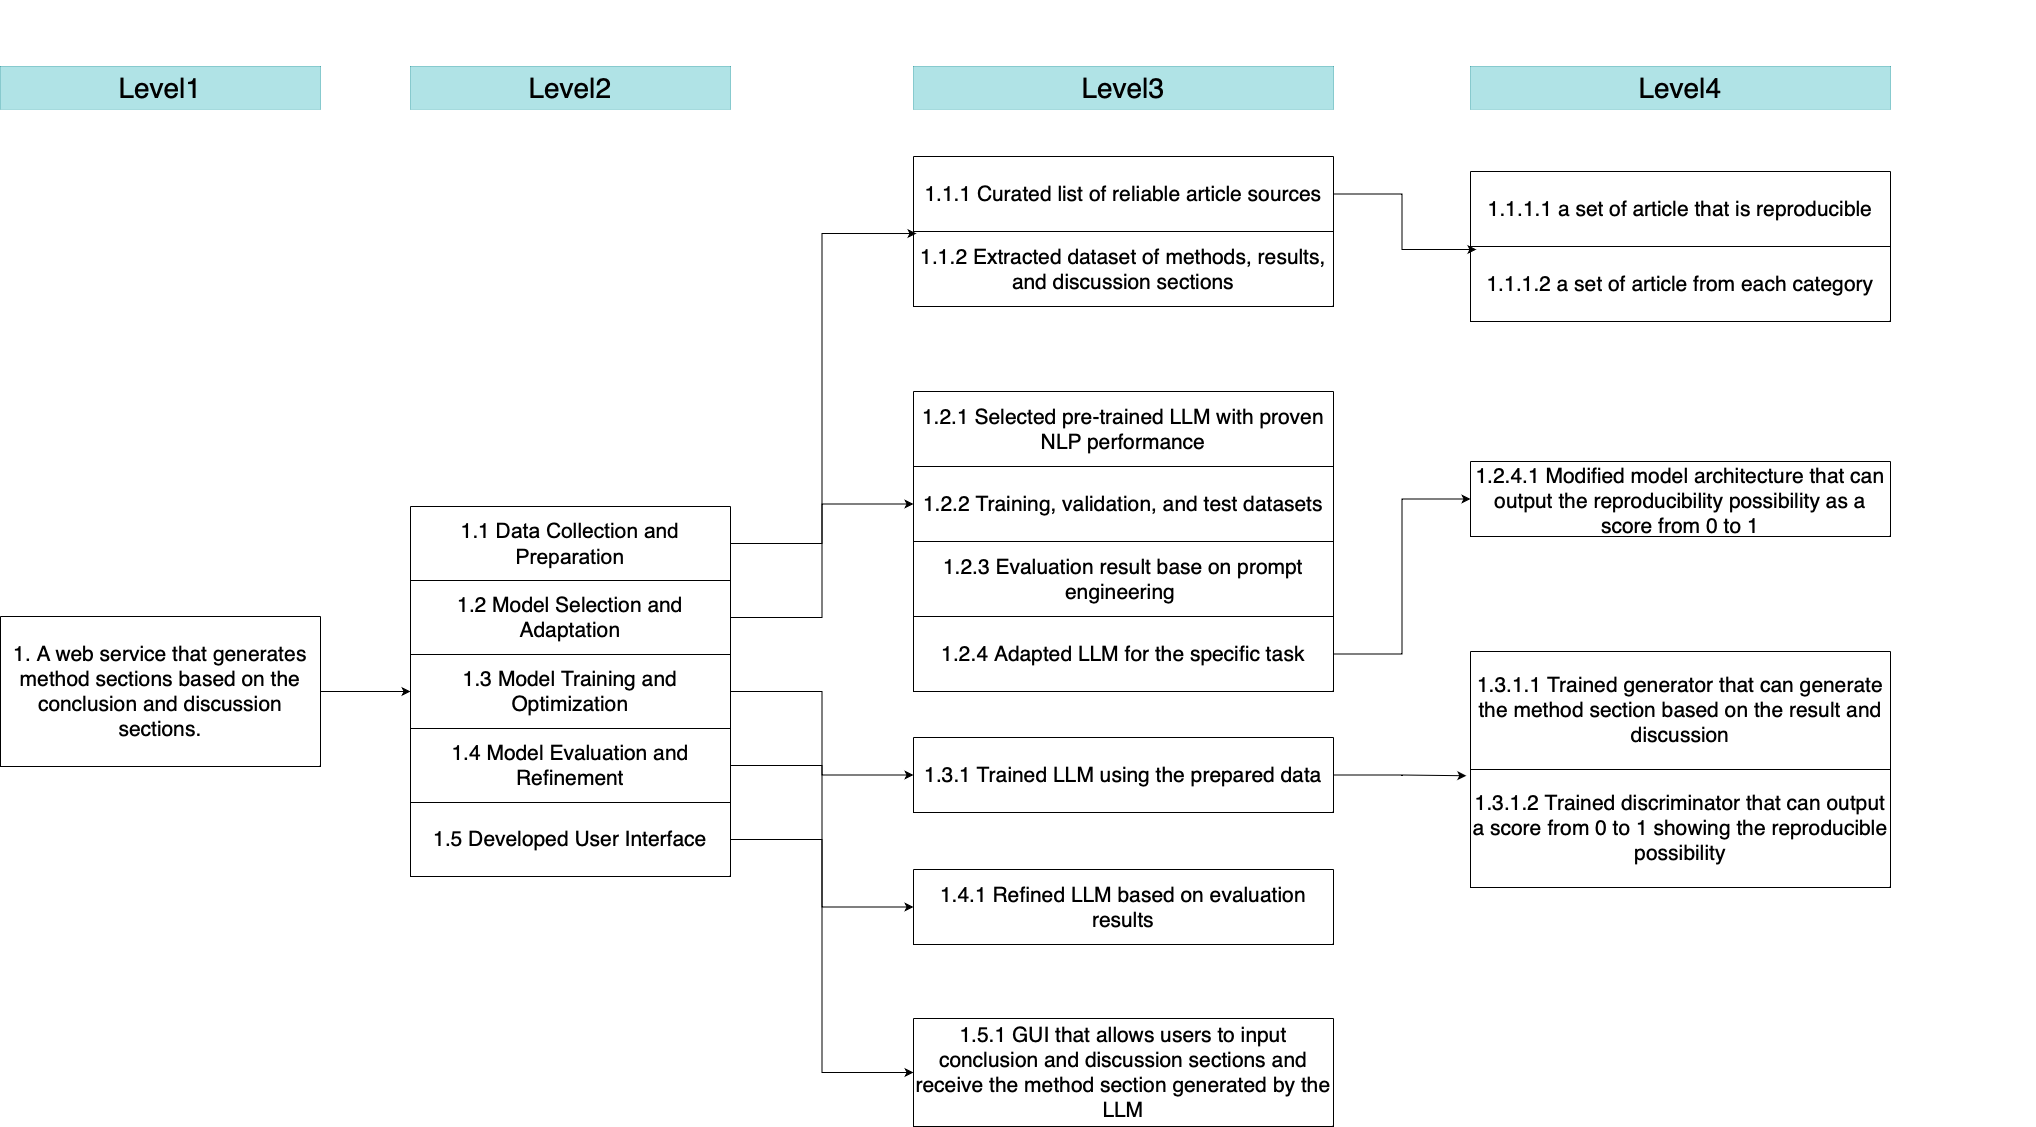
\includegraphics{wbs.png}}
				\caption[WBS Figure]{WBS Figure} 
				\label{fig:wbs}
		\end{figure*}
		\subsection{PERT}
		In order to effectively plan and manage our project, we created a PERT (Program Evaluation and Review Technique) diagram \ref{fig:pert}. This allowed us to visually map out all of the tasks and activities required for the project, as well as their dependencies and timelines. By breaking down the project into smaller, more manageable components, we were able to identify potential bottlenecks and areas where additional resources may be needed. This helped us to create a more accurate timeline for the project, as well as identify any potential risks or issues that may arise. Overall, the use of a PERT diagram was instrumental in ensuring the success of our project and keeping it on track throughout its entire lifecycle.

		\begin{figure*}[!ht]
				\centering
				\resizebox{1\textwidth}{!}{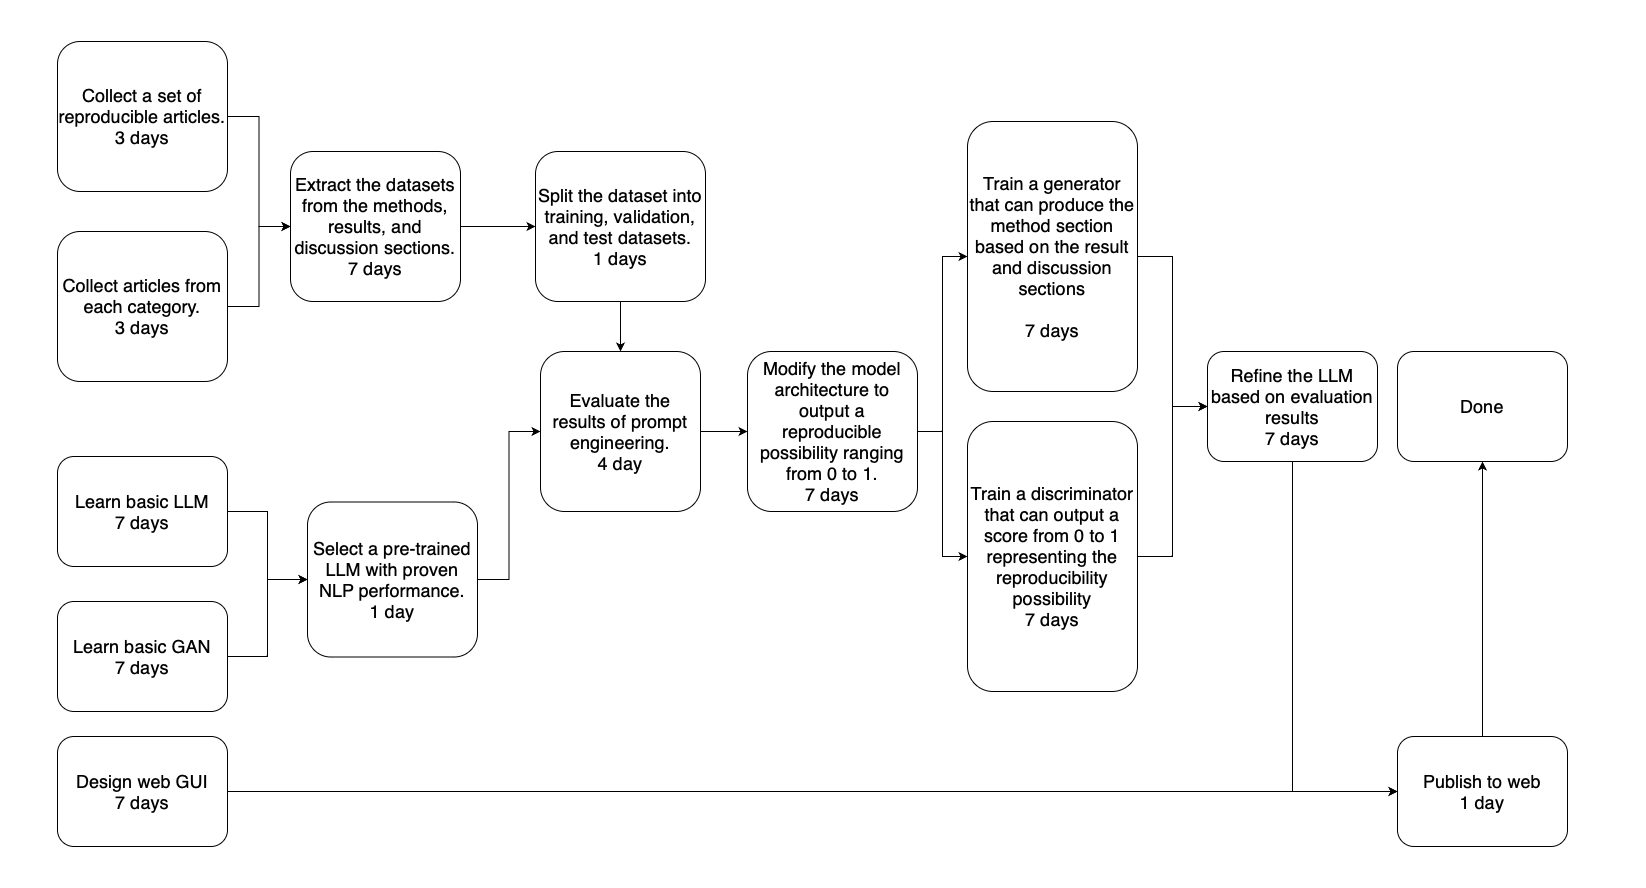
\includegraphics{pert.png}}
				\caption[PERT Figure]{PERT Figure} 
				\label{fig:pert}
		\end{figure*}

		\subsection{Gantt chart}
		In order to effectively plan and manage our project, we decided to create a Gantt chart \ref{fig:gantt}. This chart helps us to visualize the project timeline, including the start and end dates of each task, as well as dependencies between tasks. With this tool, we are able to more easily identify potential delays or roadblocks, and adjust the project plan accordingly. Additionally, the Gantt chart provides a clear and concise way to communicate the project timeline to stakeholders, ensuring that everyone is on the same page and understands what needs to be done in order to meet project goals.

		\begin{figure*}[!ht]
				\centering
				\resizebox{1\textwidth}{!}{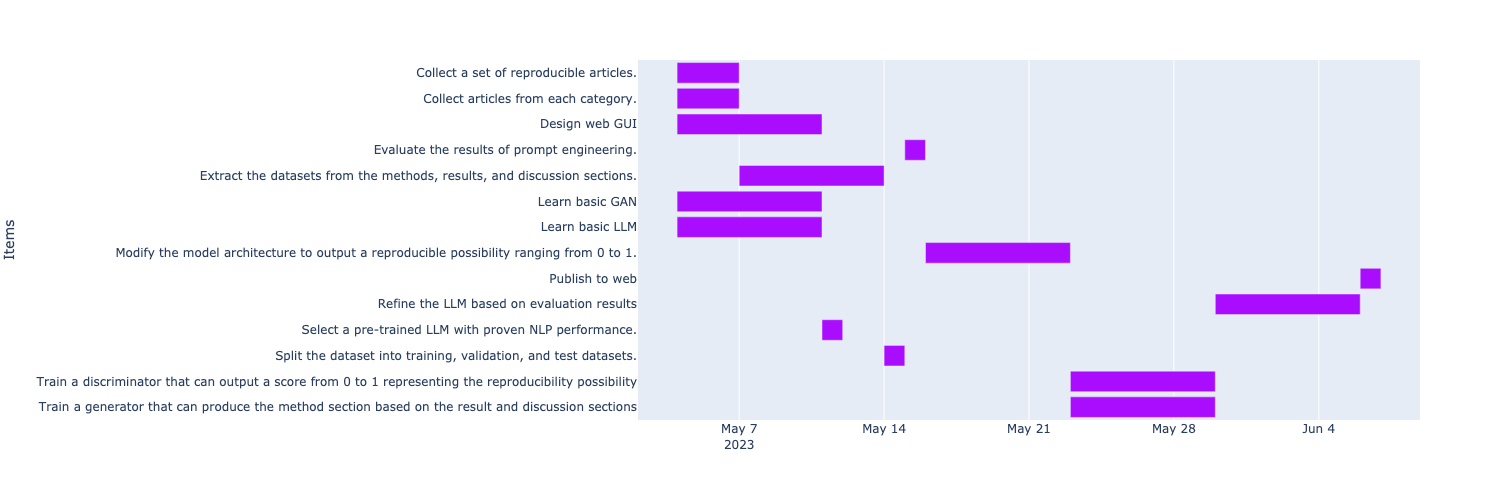
\includegraphics{gantt.png}}
				\caption[Gantt Chart Figure]{Gantt Chart Figure} 
				\label{fig:gantt}
		\end{figure*}

	
\end{document}      % End of the document
